%label:"fig:somePolyhedralComplexes"
%author:JeffHicks
%name:"examples and nonexamples of polyhedral complexes."
%type:"figure"
%parent:"con:dehnTwist"
%caption:"Two examples of unions of polyhedra. On the left, a polyhedral complex. The right figure is not an example of a polyhedral complex"

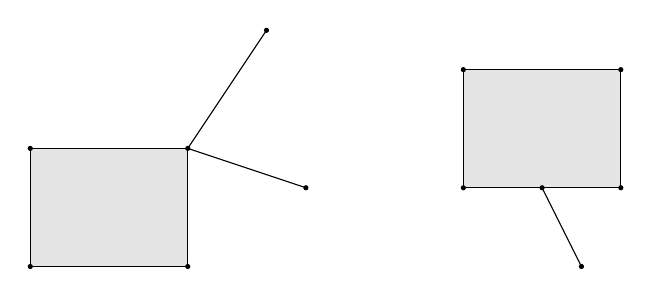
\begin{tikzpicture}\begin{scope}[]

    \draw (-1,1.5) -- (-2,0) -- (-0.5,-0.5);
    \draw[fill=gray!20]  (-4,-1.5) rectangle (-2,0);
\end{scope}\begin{scope}[shift={(5.5,1)}]

    \draw[fill=gray!20]  (-4,-1.5) rectangle (-2,0);
    \draw (-3,-1.5) -- (-2.5,-2.5);
\end{scope}
\node[fill=black, circle, scale=.2] at (-4,-1.5) {};
\node[fill=black, circle, scale=.2] at (-4,0) {};
\node[fill=black, circle, scale=.2] at (-2,0) {};
\node[fill=black, circle, scale=.2] at (-2,-1.5) {};
\node[fill=black, circle, scale=.2] at (-0.5,-0.5) {};
\node[fill=black, circle, scale=.2] at (-1,1.5) {};
\node[fill=black, circle, scale=.2] at (1.5,-0.5) {};
\node[fill=black, circle, scale=.2] at (2.5,-0.5) {};
\node[fill=black, circle, scale=.2] at (1.5,1) {};
\node[fill=black, circle, scale=.2] at (3.5,1) {};
\node[fill=black, circle, scale=.2] at (3.5,-0.5) {};
\node[fill=black, circle, scale=.2] at (3,-1.5) {};
\end{tikzpicture}

